\section{Introduction}

Particle physics research is a highly active field nowadays with a sizeable focus being placed on the development of techniques and programs to conduct numerical calculations and simulations in order to determine quantities of interest. One particular area in which I am exploring is that of the simulation of fundamental interactions of nature that we observe in particle colliders such as the Large Hadron Collider (LHC) in Geneva, Switerland. The LHC's goal is to collide protons together at sufficiently high energies that they, for lack of a better term, explode into a million particles. By observing these particles we can reconstruct factors of the interaction itself and the things that occur shortly after the collision that we don't directly see in any detectors.

\subsection{Purpose of Simulation Runs}

Simulation tools such as \textsc{MadGraph5}, \textsc{Pythia8}, and \textsc{Herwig++} are designed to simulate these interactions as closely as possible as a way to apply our current theoretical frameworks and generate results to be used to compare to experimental results as well as make predictions and fine tune our theory.

In particular, one thing that simulation tools are used for are discovering new fundamental particles. Often times, exotic particles are created in nearly identical ways to other particles. The ``signal'' representative of the processes that produce the particle of interest need to be distinguished from the ``background,'' representative of the myriad other particles created via the same or nearly identical processes. The goal is to generate enough events with enough accuracy that one can ``separate'' the signal from the background with enough statistical uncertainty to conclude that the exotic particle does indeed exist.

Naturally, one way to do this is to devise simulation runs that are fine-tuned in such a way that almost exclusively signal events are generated (usually a large amount of standard background events are already produced and stored). Of course, one has to also factor in weights that effectively scale probabilities and other results due to a higher quantity of events as compared to what would be observed in experiment, but the point that this is something we can do still stands. That way, with a large portion of signal and background events, we can reduce statistical uncertainty as much as possible. If we find a particular signal that has high separation in our simulations, we can focus attention on that signal in the experimental data to make an actual confirmation.

As an example, the leptoquark is a hypothesized particle whose existence we have yet to conclusively determine. Some of my research the previous summer was devising and programming a particular production mode (a process, in other words) for the leptoquark, in which I fine-tuned coupling parameters to even further constrain the production mode. I then generated hundreds of thousands of events specific to this model in an attempt to compare this signal with the backgrounds from other particles produced by identical or similar methods. This type of analysis takes a very long time, and it is still ongoing, so I cannot provide any concrete results, but it shows that this methodology is very standard in this field.

In summary: simulation runs are important for particle physics research because of the suitability for fine-tuning the event generation to exactly what one is looking for, leading to more efficient results and predictions that can aid in the actual discovery of new particles and new, more accurate theoretical models.



\section{Simulation Outline}

\subsection{The Process Being Simulated}

There is an unfathomable amount of physics and math that goes into the creation of simulation programs and the implementation of the possible models, processes, etc., which is completely unfeasible for a semester-long undergraduate research project conducted by one student. These software packages have been around for decades, continually undergoing upgrades and remodels, and the very existence of multiple different packages is due to the fact that each has its own shortcomings. The point I am trying to get at is that this project is very, very limited.

Originally, the intention was to program up a few simple processes, such as the interaction between two electrons or muons, and have the user specify which one. However, even programming up a single process requires a sizeable quantity of mathematical routines, physics knowledge (and programmatical implementation of this knowledge), as well as, on the more general side of things for all simulations, frameworks for handling the outputted (and inputted) data. Because of this, only one process was able to be programmed, but it is moderately inclusive. This process is the collision of two protons, their interaction via a virtual photon or $Z$ boson, and the production of a lepton pair. Having the initial state constitute protons allows the implementation of the parton distribution functions (PDFs), meaning all quarks are considered for the initial state; the intermediate boson allows implementation of electroweak and QED theory; and the final state may be composed of any lepton pair, such as $e^+/e^-$, $\mu^+/\mu^-$, or $\tau^+/\tau^-$. So while it is only one single process, it is an inclusive one, technically considering many single individual processes.

Further, there is the implementation of parton showering, which is the process by which a parton, a \textit{quark} in particular, radiates away a gluon. In the immediate aftermath of the collision, quarks have a large amount of energy, and it is favorable to drop back down to a more stable energy state, and the method by which this is achieved is gluon (or photon) radiation. In simulation terminology, this is called the \textit{parton shower}, as it typically results in a ``shower'' of additional particles. This is because the radiated gluons may decay into quark/anti-quark pairs, which may subsequently radiate, and so on.

In principle, these two may be combined such that one may occur immediately after the other. However, leptons do not interact with gluons, meaning that this is not possible for the choice of process that I have made. If it were easier, I would have implemented a process with quark final states, but the theory of the strong interactions, Quantum Chromodynamics (QCD), that governs such a process, is a significantly more complicated theory and would have been a nightmare to implement. As such, the two processes remain separate.


\subsection{Execution Instructions}

\textsc{ColSim} was made as a library, so it can be interfaced with via C++. An example main file is given in 

\begin{listing}[!ht]
\begin{minted}{cpp}
#include "ColSim/ColSim.hpp"
using namespace ColSim;
using namespace std;

#include <iostream>

int main() {
  // create the main object
  ColSimMain colsim;

  colsim.init(ColSim::ColSimMain::HARD_PROCESS);

  // start/initialize generation
  colsim.start();

  // generate events
  colsim.generateEvents(100000);
	
  // generate the plots
  colsim.generatePlots();

  // stop/deinitialize generation
  colsim.stop();
    
  return 0;
}
\end{minted}
\caption{An example main program interfacing with ColSim and generating 100000 hard scattering events.}
\label{listing:colsim-main}
\end{listing}

The user first creates a \mintinline{cpp}{ColSimMain} object and initializes it for hard scattering. In between \mintinline{cpp}{start()} and \mintinline{cpp}{stop()} commands, we generate 100000 events and also generate plots. To generate events for parton showering, one can pass in the flag \mintinline{cpp}{ColSim::ColSimMain::PARTON_SHOWER}. Both types of outputs are described in a subsequent section.

\subsubsection{Dependencies}

There are a few dependencies for \textsc{ColSim}. Of course, a C++ compiler that supports the C++11 standard is required. Building is done via CMake with the minimum required version being 3.20.

On top of that, \href{https://www.lhapdf.org/}{LHAPDF} is another dependency which is used to determine PDF values, since these cannot be calculated from first principles. \textbf{This package can only be built on a Unix-like system}. Windows is not supported for LHAPDF and therefore \textsc{ColSim}. If you are on Windows, use WSL or a virtual machine. Installation instructions for Mac and Linux are fairly straightforward, just ensure that CMake can find the necessary files.

Lastly, there is a dependence on \href{http://gnuplot.info/}{Gnuplot}, a simple plotting tool. This is available in most Linux package managers and should be easy to install for Mac users as well. Ensure that the \mintinline{bash}{gnuplot} command works.

Importantly, one needs to install at least one PDF from LHAPDF in order to operate \textsc{ColSim}. The default present in the configuration file (to be described shortly) is the ``CT18NNLO'' set. For compatibility, an older set named ``cteq6l1'' (both are case sensitive) can also be used for good results. Once LHAPDF is installed and system paths are set up correctly, you can simply type:

\begin{minted}{bash}
lhapdf install CT18NNLO
\end{minted}

or

\begin{minted}{bash}
lhapdf install cteq6l1
\end{minted}

to install these PDF sets.


\subsubsection{Compiling}

Clone the \href{https://github.com/champso1/ColSim}{repository} somewhere, and cd into it. You can then follow standard CMake building:

\begin{minted}{bash}
  mkdir build
  cd build
  cmake ..
  cmake --build .
  cmake --install .
\end{minted}

The default path for binary installation is \mintinline{cfg}{/path/to/ColSim/install}, which lies within the project directory. This way, building and running the examples are very simple. Again, ensure that CMake can find LHAPDF's files. If they were not installed to standard system paths, you can set the \mintinline{bash}{LHAPDF_ROOT_DIR} variable in your shell's environment or by passing it to cmake, i.e. like

\begin{minted}{bash}
cmake .. -DLHAPDF_ROOT_DIR=/path/to/LHAPDF
\end{minted}

to point to its installation prefix.

\subsubsection{Examples}

In the \mintinline{cfg}{examples} subdirectory is an example called \mintinline{cfg}{basic}. Cd'ing into it gives the above C++ code which can be built via the standard CMake procedure. After building, an executable called \mintinline{cfg}{basic} will be in the build folder. Some things to play around with are the number of generated events, and switching to parton showering and seeing that output. Configuration file settings can also be changed -- this is described in the next section.

\subsubsection{Configuration File}

The last thing is that a configuration file is required by \textsc{ColSim}. When initializing the \mintinline{cpp}{ColSimMain} via the \mintinline{cpp}{init()} method, one can pass in the path to the configuration file. If the configuration file is in the same directory as the executable and called `config.in', you can omit this parameter -- this is the recommended thing to do. In the \mintinline{cfg}{res} folder in the top level of the project is a default configuration file containing the following information:

\begin{listing}[!ht]
  \begin{minted}{cfg}
# Center-of-Mass energy: measured in TeV
ECM=14.0

# pdf information
PDFName=CT18NNLO
PDFMemberNo=0

# ---------------------------
# ----- Hard Scattering -----
# ---------------------------
Process=PP2Zg2ll

# number of evaluations of the differential cross section in the Monte Carlo integration
NumXSIterations=1000000
  \end{minted}
  \caption{An example of a ColSim configuration file.}
  \label{listing:colsim-config-file}
\end{listing}

This can then be copied to the same place as the executable. The description of the values are:

\begin{itemize}
\item \textbf{ECM}: The center-of-mass energy of the collision. In other words, each proton has energy $\mathrm{ECM}/2$.
\item \textbf{PDFName}: The name of the PDF set to use.
\item \textbf{PDFMemberNo}: Some PDFs have multiple sets within them, usually 0 is used, but sometimes other values are used, so this is left configurable.
\item \textbf{Process}: The hard scattering process to simulate. At the moment this is the only value, so it cannot be changed.
\item \textbf{NumXSIterations}: Number of Monte Carlo iterations to do. The current default gives a good middle-ground between speed and accuracy, but can be configured if higher speed or accuracy is desired.
\end{itemize}

As an important note: the PDF information given must match that of a PDF that you have installed. 


\subsubsection{Outputs}\label{sec:outputs}

Once the example is built and the configuration file filled, you can run the executable (named `basic') and, in the case of Listing~\ref{listing:colsim-main}, a file titled `events.dat' will be created containing data for all of the generated events. In particular, the first ten lines of the file are shown in Listing~\ref{listing:events-dat}.

\begin{listing}[!ht]
\begin{minted}{text}
#cos(theta)	rho	y (rapidity)	Q	x1	
-0.951787	1.5357	0.498004	325.786	0.0229237	
-0.0794975	0.846551	0.0443711	87.5763	6.13877e-05	
-0.83998	1.21204	0.64568	114.893	0.0332578	
-0.138378	1.36989	0.107851	145.865	0.00029054	
-0.164968	0.418056	0.0662585	72.106	5.3322e-05	
-0.737887	0.668366	0.0813915	80.2655	7.61546e-05	
-0.4515	0.854714	0.667957	87.9612	0.0344976	
0.565371	0.49181	0.186333	74.3544	0.000198658	
-0.194654	0.830988	0.885909	86.8572	0.313566	
\end{minted}
\caption{The first ten lines of 'events.dat,' the output file from the hard scattering simulation.}
\label{listing:events-dat}
\end{listing}

Each row constitutes a single event with five values separated by tabs. The top line indicates the variable each column represents. In particular, the first column is $\cos\theta$, the angle between the beam axis and the first emitted lepton, the second is $\rho$, a variable with no real physical interpretation (it is an intermediate variable, in a sense, used to make calculations a bit easier) but is plotted for consistency's sake, the third is $y$, which is the rapidity and roughly corresponds to the speed of the first emitted lepton in the direction of the beam axis, the fourth is $Q$, then energy of the reaction (not the same as the center-of-mass energy in the config file), and the last is $x1$, the momentum fraction of the proton the first quark contains.

\begin{figure}[ht]
  \centering
  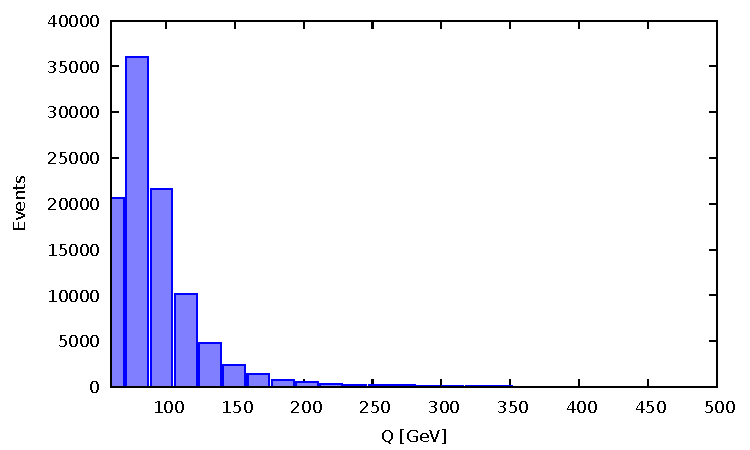
\includegraphics[width=0.4\linewidth]{./res/Images/Q.pdf}
  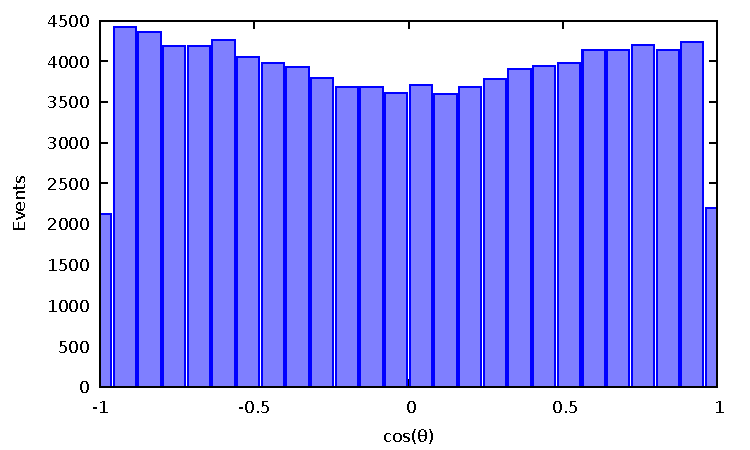
\includegraphics[width=0.4\linewidth]{./res/Images/cos_theta.pdf}
  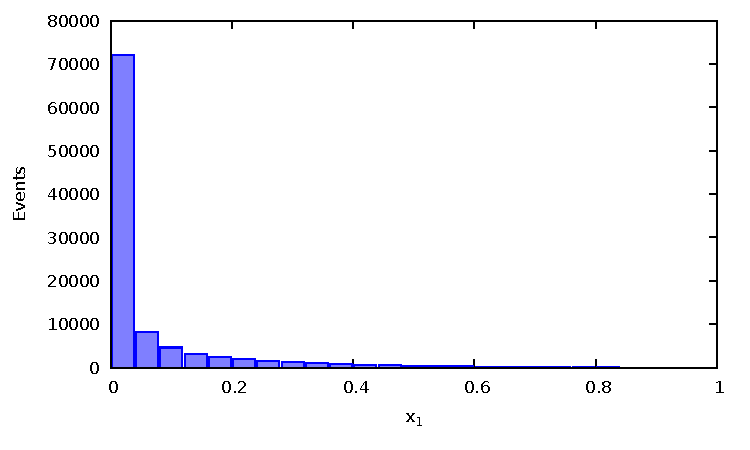
\includegraphics[width=0.4\linewidth]{./res/Images/x1.pdf}
  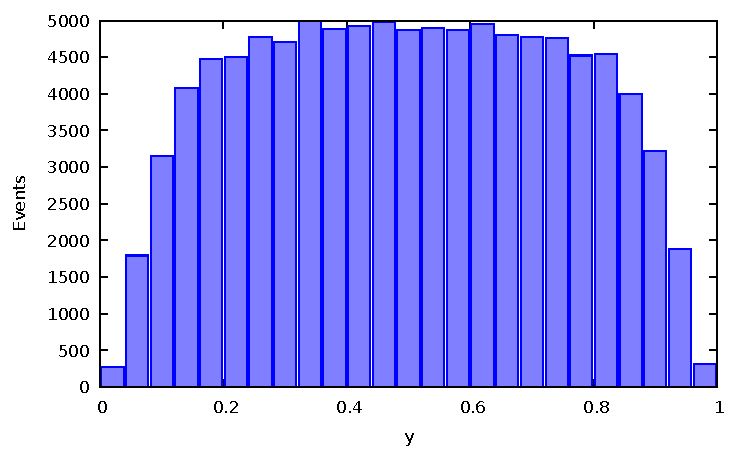
\includegraphics[width=0.4\linewidth]{./res/Images/y.pdf}
  \caption{Outplot plots for distribution of the kinematic/phase space variables for the generated hard scattering events.}
  \label{fig:q-dist}
\end{figure}

Also outputted are five plots, placed in the 'plots' directory in the build folder (or wherever the 'basic' executable is), which are histograms of the above quantities, in which the $x$-axis corresponds to the value of the variable and the $y$-axis corresponds to the number of events in that bin. Plots of $\cos\theta$ and $Q$ are given in Fig.~\ref{fig:q-dist}.

Changing the initialization flag in the program to instead do the parton showering, the same idea applies: a file, this time called 'emissions.dat' will be created that contains as rows each generated event, and each column corresponds to a particular variable. The first ten lines of this output file are given in Listing~\ref{listing:emissions-dat}

\begin{listing}[!ht]
\begin{minted}{text}
#t	pT	m
31.1053	10.1835	17.7978	
14.6723	6.68227	9.90174	
25.9178	6.50954	12.9889	
18.2344	2.75489	7.08758	
18.2067	6.32354	10.7299	
22.1597	7.11254	12.5543	
18.3092	3.78753	8.32746	
25.3827	6.36348	12.7091	
20.8469	4.96856	10.1774	
\end{minted}
\caption{The first ten lines of 'emissions.dat,' the output data file for parton showering simulation.}
\label{listing:emissions-dat}
\end{listing}

Here, $t$ is the scale at which the emission occurred, $p_T$ is the square of the transverse momentum of the emitted gluon, and $m$ is the square of the virtual mass of the emitted gluon, since the gluon is technically massless, but due to special relativity one can interpret its energy as a mass.

\begin{figure}[ht]
  \centering
  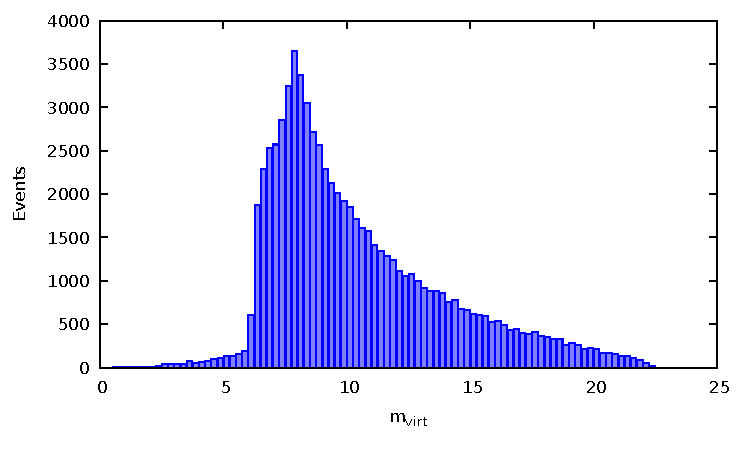
\includegraphics[width=0.4\linewidth]{./res/Images/m.pdf}
  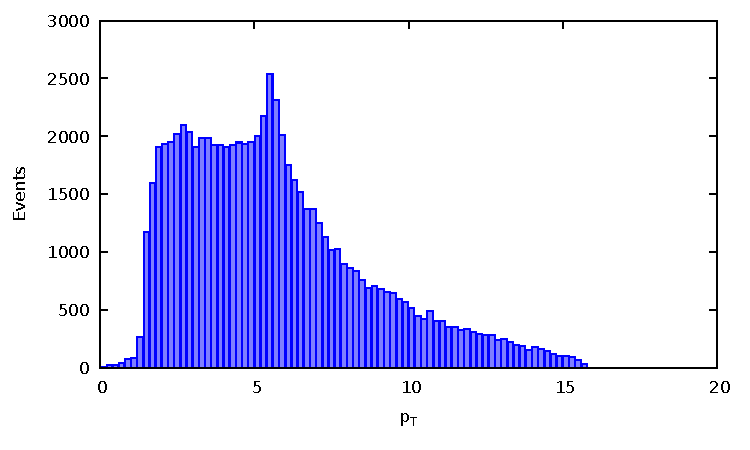
\includegraphics[width=0.4\linewidth]{./res/Images/pT.pdf}
  \caption{Output plots for $m^2$ and $p_T^2$ for the generated parton showering events.}
  \label{fig:partonshower-dist}
\end{figure}

In Fig.~\ref{fig:partonshower-dist} are the generated plots for the $pT$ and $m$ distributions for the generated parton showering events, with the same scheme for the $x$ and $y$-axis as for the hard scattering events. What we notice is that there are very few events generated below a particular threshold, and after we pass that threshold, there is a spike of generated events, followed by a falloff as the energy increases. This is exactly what we expect: the Sudakov form factor, if we recall, is the probability that we can evolve the parton from energy $t_0$ to $t$ \textit{without} emission. What this essentially indicates is that there is a higher probability of emission at lower scales simply due to the fact that it has spent more time without an emission. Further, the reason for the apparent sharp threshold at $\sim\qty{5}{\giga\electronvolt}$ is because we only evolve down to a certain energy. This is because our theory of the strong interaction, by which this process is governed, breaks down at those energies. We could choose to evolve right down to $\qty{0}{\giga\electronvolt}$, but of course results below the threshold should be ignored as they are guaranteed to be inaccurate.


\subsection{Assumptions/Limitations}

As I've mentioned already, the scope of this project is extremely limited. In particular, there is only one process that may occur at the hard scattering scale and one process that may occur at the parton showering scale. This of course means that, in some sense, I'm not actually simulating what I want to simulate, since I'm not including everything that we know happens in such a process. However, I \textit{am} simulating a very plausible (and in fact very \textit{likely}, as well) \textit{piece} of what actually happens at such a process. So, while there may be few pieces and they may not be connected, they are still large pieces in the puzzle.

That being said, there are a couple more considerations: often times, quantities determined in calculations are dependent on one or possibly two scales, those being the \textit{factorization scale} $\mu_f$ and the \textit{renormalization scale} $\mu_r$. One such quantity is the coupling ``constant''\footnote{It being called a ``constant'' is an unfortunate remnant of a time before its non-constantness was discovered.}. Without too much loss of precision, one may keep this fixed at a generic scale often taken to be the energy of the process under consideration, or the mass of the Z boson, etc., or one may choose to vary it, in which additional considerations have to be taken. In my project, it is taken constant.

\subsection{Side Comments}

As a side note, some feedback on a previous milestone which presumably lost me a few points was the fact that some physical quantities were hardcoded and not left up to configuration. This is because approximately 95\% of the quantities in the Constant.hpp file are genuine constants, and cannot be changed. This would be like me hard coding the value of the acceleration due to gravity for a simulation done on Earth. \textit{Sure}, we \textit{could} leave it up to the user to configure how they like, but any results other than what would have been originally hard coded should be completely ignored for the obvious reason that the results of the simulation would not representative of the actual process under consideration. I suppose it is partly on me for assuming this knowledge, but I hope this has been clarified.

While I'm already making a side comment about the aforementioned feedback, there was also a comment about missing references to some physics formulas presented in the literature review. I did indeed reference them, though I did delegate it to a footnote, so it may have been missed. To reiterate: all results presented in the beginning part of the literature review are highly common knowledge in the realm of physics, and everything can be found in any generic textbook on the subject, such as ``Introduction to Quantum Field Theory'' by Peskin and Schroeder~\cite{peskin-schroeder}. The same can be said for the Monte Carlo algorithm. From some basic searches indicate that the original algorithm has no associated publication, but, similarly to before, it and some of the other generic mathematical routines can be found in any computational physics textbook, such as ``Numerical Recipes'' by William Press~\cite{Press_2007}. The specific methods for the parton showering was cited at the beginning of the section. I hope this has cleared up any confusion.



\section{Simulation Runs}

This section essentially aligns with what I have already described back in Section~\ref{sec:outputs}, so I refer discussion of these topics to there. There is no need for a table, since there is only one particular thing to simulate, and the outputs/motivations/etc. are given in that section (and the introduction).



\section{Data Collection and Storage}

Data is stored very simply. After the production of each event, the corresponding quantities of interest or organized into an array which is returned to the calling function. An ``event record'' is accumulated with $N$ arrays corresponding to the $N$ generated events. At the end of the program, all of this data is dumped to a .dat file which is stored in a way that Gnuplot can handle. In particular, each array occupies its own line, with each entry in each line separated by a tab. A comment at the top of the file indicates the column names.

No preprocessing is necessary on the data. More could be done, but it is not necessary.


\section{Changes/Considerations Since Proposal}

Here I briefly outline some of the major changes and other consideration that I have made to the project compared to what was presented in the proposal. I've littered some of this description throughout this document so far, and also updated the original proposal/literature review document to reflect these changes, but I'll list them out concretely.

First, I will not be implementing more than a single hard process and a single type of showering, that being $pp \rightarrow Z/\gamma^* \rightarrow \ell^+\ell^-$ and gluon radiation, respectively. The motivation for the latter is simple, and it is that photon emission is a very different game compared to gluon emission, and numerous new physics and mathematical effects are at play. The former is simply due to time constraints; the given process is very inclusive, meaning it is representative of a number of different similar process involving the electroweak force, but any other process would be in a different framework and thus require a good deal of additional programming. Fortunately, the inclusivity of this process still provides very nice results. Further, by virtue of how the calculations are carried out, additional process are exactly that: additional process. They simply add together to get a more full result, but don't necessarily impact each other.

Second, I originally had planned to be able to connect the hard scattering and parton showering together, meaning I could generate events from the hard scattering reaction and immediately shower them, but the showering is only implemented for quarks radiating gluons, and the final state of the events from the hard scattering process are leptons. I would have to either implement a QCD process or photon emission, both of which are a bit more challenging than what I have currently implemented. Therefore, these are two separate parts of the program.

Lastly, the initial plan to use LHE files to interact with other programs is limited as well. The defaults for LHE files that other programs to accept and spit out is quite involved, and in order for me to successfully implement those things, it would require a significant amount of work. Because of this, interoperabillity with \textsc{Madgraph5} and \textsc{Pythia8} is limited to only simple/qualitative comparisons of their output data.

Apart from this, the underlying simulation structure attributed to Monte Carlo integration and the Sudakov form factor is still the same, as well as the general structure of the program. No additional dependencies were required\footnote{I did mention GSL in a previous milestone, but I have implemented the necessary mathematical routines myself, so this dependency is for sure out of the equation.}

\section{Next Steps}

There are two main things I want to work on next. While I did mention earlier that 95\% of the physical constants are hard-coded due to their nature, i.e. that changing them would inherently give results that are not desirable for comparison with experiment which, at the end of the day, is the point of simulations. However, allowing control of some\footnote{Only \textit{some}; about 80\% of the parameters are genuine constants, and changing them would make no sense at all, like changing gravity for a simulation conducted on Earth.} parameters would be nice to gain an understanding of how the simulation responds to changes in those parameters.

The other thing is the implementation of LHE file output first, and input later. Input would have to be extremely specific to simple processes with final states that are quarks, which, as mentioned earlier, is very challenging with existing simulation tools. Outputs would be nice, particularly for the hard scattering process, since I could feed those into \textsc{Pythia8} and see what happens.

As a third, less pertinent step, general cleanup of the code would be in order, particularly with the plotting interface, but it is perfectly servicable at the moment so this has a very low priority.



\section{Conclusions/Discussion}

To provide a conclusion, it is evident that the simulation is performing very well. The speed is very nice, taking only a few seconds to do millions of cross section evaluations and hundreds of thousands of events generated. Additionally, the generated results are exactly what is expected based on physics knowledge.


\section{Documentation Updates}

There have been only a handful of changes to the documentation, but those have been discussed already in the corresponding sections in this paper. I have updated the literature review/model details document to reflect these changes.






%%% Local Variables:
%%% mode: LaTeX
%%% TeX-master: "../../Milestone5"
%%% End:
